%beamer

%\PassOptionsToClass{handout}{beamer}

% \newboolean{handoutmode}
% \setboolean{handoutmode}{false}
%\newcommand{\handoutmode}{}

%% LaTeX-Beamer template for KIT design
%% by Erik Burger, Christian Hammer
%% title picture by Klaus Krogmann
%%
%% version 2.1
%%
%% mostly compatible to KIT corporate design v2.0
%% http://intranet.kit.edu/gestaltungsrichtlinien.php
%%
%% Problems, bugs and comments to
%% burger@kit.edu
\ifdefined \handoutmode
\documentclass[18pt, handout]{beamer}
\else
\documentclass[18pt]{beamer}
\fi

\usepackage[T1]{fontenc}
\usepackage[utf8]{inputenc}

\usepackage{../preamble/templates/beamerthemekit}

\usepackage[vlined]{algorithm2e}  %possible: noend, noline, ...
\usepackage{amssymb}
\usepackage{amsmath}
\usepackage{wasysym}
\usepackage{graphicx}
%\usepackage{hyperref}
\usepackage[export]{adjustbox}
\usepackage{wrapfig}
\usepackage{colortbl}
\usepackage{tikz}
\usetikzlibrary{matrix}
\usetikzlibrary{arrows.meta}
\usetikzlibrary{automata}
\usetikzlibrary{tikzmark}
\graphicspath{{images/}}
%\usepackage[colorlinks=true,urlcolor=blue,linkcolor=blue]{hyperref}
\usepackage[outline]{contour}
\usepackage{cancel}
\usepackage[warn]{textcomp}
\usepackage{multicol}
\usepackage{tabularx}
\usepackage{xcolor}
\usepackage{hhline}
\usepackage{environ}
\usepackage{calc}
\usepackage{bm}
\usepackage{xspace} % for \xspace command
\usepackage{varwidth}
\usepackage{csquotes}

\newcommand{\mycomment}[1]{}

%%%% CONFIG

\input{../preamble/config.tex}

%%%% CONFIG END

%\renewcommand{\SS}{\iffontchar\font"1E9E \symbol{"1E9E}\else SS\fi} % SHAME ON YOU, LATEX!
\newcommand{\TM}{\text{$\mbox{}^\text{\tiny TM}$}}
\newcommand{\pluseq}{\mathrel{+}=}
\newcommand{\pp}{\operatorname{++}} 
\newcommand{\mm}{\operatorname{--\mbox{\:}--}}
\newcommand{\minuseq}{\mathrel{-}=}
\newcommand{\asteq}{\mathrel{*}=}
\newcommand{\muleq}{\asteq}
\renewcommand{\mod}{\mathop{\textbf{mod}}} 
\renewcommand{\div}{\mathop{\textbf{div}}}
\newcommand{\N}{\mathbb{N}} 
\newcommand{\R}{\mathbb{R}}
\newcommand{\Z}{\mathbb{Z}}
\newcommand{\E}{\mathbb{E}}
\renewcommand{\P}{\mathbb{P}}
\newcommand{\BB}{\mathbb{B}} % \B already exists
\newcommand{\NP}{\ensuremath{\mathcal{N\hspace{-1.5pt}P}}}
\newcommand{\Oh}[1]{\mathcal{O}\!\left(#1\right)}
\renewcommand{\O}{\mathcal{O}}
\newcommand{\Om}[1]{\Omega\!\left(#1\right)}
\newcommand{\Th}[1]{\Theta\!\left(#1\right)}

\newcommand{\realTilde}{\textasciitilde\xspace}
\renewcommand{\qedsymbol}{\textcolor{black}{\openbox}}

\newcommand{\size}[1]{\ensuremath{\left\lvert #1 \right\rvert}}
\newcommand{\set}[1]{\left\{#1\right\}}
\newcommand{\tuple}[1]{\left(#1\right)}

\newcommand*{\from}{\colon}

\newcommand{\morescalingdelimiters}{   % for proper \left( \right) typography
	\delimitershortfall=0pt  % formerly: 0pt  
	\delimiterfactor=1
}
% todo later
%\delimitershortfall=0pt  % for proper \left( \right) typography
%\delimiterfactor=1

% --- \frameheight constant ---
\newlength\fullframeheight
\newlength\framewithtitleheight
\setlength\fullframeheight{.92\textheight}
\setlength\framewithtitleheight{.86\textheight}

\newlength\frameheight
\setlength\frameheight{\fullframeheight}

\let\frametitleentry\relax
\let\oldframetitle\frametitle
\def\frametitle#1{\global\def\frametitleentry{#1}\if\relax\frametitleentry\relax\else\setlength\frameheight{\framewithtitleheight}\fi\oldframetitle{#1}}

% --- \frameheight constant end ---

\def\·{\cdot}
\def\*{\cdot}
\def\<{\langle}
\def\>{\rangle}


\newcommand{\zB}{z.\,B.\@\xspace}
\newcommand{\ZB}{Z.\,B.\@\xspace}

\newcommand{\ceil}[1]{\left\lceil#1\right\rceil}
\newcommand{\floor}[1]{\left\lfloor#1\right\rfloor}
\newcommand{\abs}[1]{\left|#1\right|}
\newcommand{\Matrix}[1]{\begin{pmatrix} #1 \end{pmatrix}}
\newcommand{\braced}[1]{\left\lbrace #1 \right\rbrace}
\newcommand{\llist}[1]{\langle #1 \rangle}
\newcommand{\Mid}{\;\middle|\;}

\let\after\circ

\newcommand{\entspr}{\ensuremath{\mathrel{\hat{=}}}\xspace}

\def\~~>{\ensuremath{\rightsquigarrow}}  % FuCKING FINALLY! :D

% "something" placeholder. Useful for repairing spacing of operator sections, like `\sth = 42`.
\def\sth{\vphantom{.}}

\def\fract#1/#2 {\frac{#1}{#2}}  % ! TRAILING SPACE is CRUCIAL!
\def\dfract#1/#2 {\dfrac{#1}{#2}} % ! Trailing space is crucial!

\newcommand{\tight}[1]{{\renewcommand{\arraystretch}{0.76} #1}}
\newcommand{\stackedtight}[1]{{\renewcommand{\arraystretch}{0.76} \begin{matrix} #1 \end{matrix}} }
\newcommand{\stacked}[1]{\begin{matrix} #1 \end{matrix} }
\newcommand{\casesl}[1]{\delimitershortfall=0pt  \left\lbrace\hspace{-.3\baselineskip}\begin{array}{ll} #1 \end{array}\right.}
\newcommand{\casesr}[1]{\delimitershortfall=0pt  \left.\begin{array}{ll} #1 \end{array}\right\rbrace}
\newcommand{\caseslr}[1]{\delimitershortfall=0pt  \left\lbrace\begin{array}{ll} #1 \end{array}\hspace{-.3\baselineskip}\right\rbrace}

\def\q#1uad{\ifnum#1=0\relax\else\quad\q{\the\numexpr#1-1\relax}uad\fi}
% e.g. \q1uad = \quad, \q2uad = \qquad etc.

\newcommand{\qqquad}{\q3uad}


\def\indentstring{}
\def\§#1{\def\indentstring{#1}#1}
\def\.{{$\hphantom{\text{\indentstring}}$}}


\newcommand{\impl}{\ifmmode\ensuremath{\mskip\thinmuskip\Rightarrow\mskip\thinmuskip}\else$\Rightarrow$\xspace\fi}  
\newcommand{\Impl}{\ifmmode\implies\else$\Longrightarrow$\xspace\fi}

\newcommand{\gdw}{\ifmmode\mskip\thickmuskip\Leftrightarrow\mskip\thickmuskip\else$\Leftrightarrow$\xspace\fi}
\newcommand{\Gdw}{\ifmmode\iff\else$\Longleftrightarrow$\xspace\fi}

\newcommand{\symbitemnegoffset}{\hspace{-.33\baselineskip}}
\newcommand{\implitem}{\item[\impl\symbitemnegoffset]}
\newcommand{\Implitem}{\item[\Impl\symbitemnegoffset]}


\newcommand{\forcenewline}{\mbox{}\\}

\newcommand{\bfalert}[1]{\textbf{\alert{#1}}}
\let\elem\in   % I'm a Haskell freak. Don't judge me. :P


\newenvironment{threealign}{%
	\[
	\begin{array}{r@{\ }c@{\ }l}
}{%
	\end{array}	
	\]
}


\makeatletter
% Provides color if undefined.
\newcommand{\colorprovide}[2]{%
	\@ifundefinedcolor{#1}{\colorlet{#1}{#2}}{}}
\makeatother



%\pgfdeclarelayer{background}
%\pgfdeclarelayer{foreground}
%\pgfsetlayers{background,main,foreground}

\colorprovide{lightred}{red!30}
\colorprovide{lightgreen}{green!40}
\colorprovide{lightyellow}{yellow!50}
\colorprovide{beamerlightred}{lightred}
\colorprovide{beamerlightgreen}{lightgreen}
\colorprovide{beamerlightyellow}{lightyellow}
\colorprovide{fullred}{red!60}
\colorprovide{fullgreen}{green}
\definecolor{darkred}{RGB}{115,48,38}
\definecolor{darkgreen}{RGB}{48,115,38}
\definecolor{darkyellow}{RGB}{100,100,0}

\only<handout:0>{\colorlet{adaptinglightred}{beamerlightred}}
\only<handout:0>{\colorlet{adaptinglightgreen}{beamerlightgreen}}
\only<handout:0>{\colorlet{adaptinglightyellow}{beamerlightyellow}}
\only<beamer:0>{\colorlet{adaptinglightred}{lightred}}
\only<beamer:0>{\colorlet{adaptinglightgreen}{lightgreen}}
\only<beamer:0>{\colorlet{adaptinglightyellow}{lightyellow}}
\only<handout:0>{\colorlet{adaptingred}{lightred}}
\only<beamer:0>{\colorlet{adaptingred}{fullred}}
\only<handout:0>{\colorlet{adaptinggreen}{lightgreen}}
\only<beamer:0>{\colorlet{adaptinggreen}{fullgreen}}

\colorlet{checkgreen}{green!80}
\colorlet{crashred}{fullred}
\colorprovide{myalertcolor}{red}
\colorlet{alertcolor}{myalertcolor}

\definecolor{kwblue}{rgb}{0.3,0.3,1}
\definecolor{strcolor}{RGB}{48,115,38}

\newcommand{\str}[1]{\shorthandoff{"}\textcolor{strcolor}{\text{"{}#1"{}}\shorthandon{"}}}

\newcommand{\gray}[1]{\textcolor{gray}{#1}}

\newcommand{\MyKwSty}[1]{\textcolor{kwblue}{\textbf{#1}}}
\SetKwSty{MyKwSty}

\SetArgSty{textnormal} % to end conditional italics madness

\newcommand{\MyCommentSty}[1]{\emph{\gray{#1}}}
\SetCommentSty{MyCommentSty}

\SetKwComment{Comment}{// }{}

\newcommand{\LComment}[1]{\Comment*[h]{#1}}
\newcommand{\RComment}[1]{\quad \Comment*[h]{#1}}



\SetKwBlock{KwFunc}{function}{}
\SetKwBlock{KwProc}{procedure}{}
\newcommand{\Function}[2]{\KwFunc({#1}){#2}}
\newcommand{\Procedure}[2]{\KwProc({#1}){#2}}
\SetKwBlock{KwEmptyBlock}{}{}
\newcommand{\EmptyBlock}[1]{\KwEmptyBlock(){#1}}

% Binary operator keywords (small surrounding spaces)
\newcommand{\SetKwBin}[2]{
	\expandafter\newcommand\csname #1\endcsname{\ensuremath{\mathbin{\KwSty{#2}}}}	
}
% Relational operator keywords (bigger surrounding spaces)
\newcommand{\SetKwRel}[2]{
	\expandafter\newcommand\csname #1\endcsname{\ensuremath{\mathrel{\KwSty{#2}}}}	
}
% Directive keywords (trailing space)
\newcommand{\SetKwDir}[2]{
	\expandafter\newcommand\csname #1\endcsname{\ensuremath{\mathop{\KwSty{#2}}}}		
}

\DontPrintSemicolon
%\SetKwSwitch{Switch}{Case}{Other}{switch on}{}{}{else}{}{}

%\newcommand{\SwitchCase}[2]{\KwSty{case} #1 \KwOf\EmptyBlock{#2}}
%\newcommand{\case}[2]{#1:\EmptyBlock{#2}}
\SetKwDir{KwAssert}{assert}
\SetKwDir{KwInvariant}{invariant}
\SetKwRel{KwStep}{step}
\SetKwRel{KwDownto}{downto}	
\SetKwDir{KwArrayOf}{array of\,}
\SetKwDir{KwArray}{array}
\let\KwTo\undefined
\SetKwRel{KwTo}{to}
\SetKwRel{KwOf}{of}
\let\KwInput\KwIn
\let\KwIn\undefined
\SetKwRel{KwIn}{in}
\SetKwRel{KwInto}{into}
\SetKwDir{KwNot}{not}
\SetKwRel{KwIs}{is}
\SetKwRel{KwAnd}{and}
\SetKwRel{KwOr}{or}
\SetKwBin{KwMod}{mod}
\SetKwBin{KwDiv}{div}
\SetKwDir{KwContinue}{continue}
\SetKwDir{KwBreak}{break}
\SetKwDir{KwThrow}{throw}
\SetKw{KwTrue}{true}
\SetKw{KwFalse}{false}
\SetKw{KwThis}{this}
\SetKwDir{KwNew}{new}
\SetKwRel{KwFrom}{from}
\SetKwDir{KwFor}{for}
\SetKwDir{KwEach}{each}
\SetKw{KwProcedure}{procedure}
\SetKw{KwMethod}{method}
\SetKw{KwFunction}{function}
\SetKwDir{KwPointerTo}{Pointer to}
\SetKwData{KwList}{List}
\SetKwData{KwSet}{Set}
\newcommand{\Element}{\|Element|}
\newcommand{\KwListOf}{\ensuremath{\mathop{\KwList \KwOf}}} 
\newcommand{\KwSetOf}{\ensuremath{\mathop{\KwSet \KwOf}}} 
\SetKwDir{KwDispose}{dispose}


\def\|#1|{\text{\normalfont #1}}  % | steht für senkrecht (anstatt kursiv wie sonst im math mode)

% proper math typography
\newcommand{\functionto}{\longrightarrow} 
\renewcommand{\geq}{\geqslant}
\renewcommand{\leq}{\leqslant}
\let\oldsubset\subset
\renewcommand{\subset}{\subseteq} % for all idiots out there using subset

\newcommand{\access}{\text{\textrightarrow}} 
\def\->{\access}

\let\oldemptyset\emptyset
\let\emptyset\varnothing % proper emptyset

\newcommand{\stdarraystretch}{1.20}
\renewcommand{\arraystretch}{\stdarraystretch}  % for proper row spacing in tables

\newcommand{\mailto}[1]{\href{mailto:#1}{{\textcolor{blue}{\underline{#1}}}}}
\newcommand{\urlnamed}[2]{\href{#1}{\textcolor{blue}{\underline{#2}}}}
\renewcommand{\url}[1]{\urlnamed{#1}{#1}}

\newcommand{\hanging}{\hangindent=0.7cm}
\newcommand{\indented}{\hanging}

\newcommand{\Pros}{{\huge \protect\textcolor{adaptinggreen}{\protect\contour{black}{\raisebox{-.3pt}{$\protect\textbf{+}$}}}}\xspace}

\newcommand{\Cons}{\hspace{1pt}\protect\scalebox{0.88}[1]{\huge \protect\contour{black}{\protect\textcolor{adaptingred}{\raisebox{-1pt}{$\protect\textbf{--}$}}}}\hspace{1pt}\xspace}

\newcommand{\yop}{\textcolor{checkgreen}{\protect\contour{black}{\protect\textbf{\checked}}}\xspace}
\newcommand{\crash}{\ensuremath{\textcolor{crashred}{\protect\contour{black}{\protect\textbf{\lightning}}}}\xspace}

\newcommand{\YesCellE}[1]{\cellcolor{adaptinggreen} {#1}}
\newcommand{\YesCell}{\YesCellE{\textbf{Ja}}}
\newcommand{\NoCellE}[1]{\cellcolor{adaptingred} {#1}}
\newcommand{\NoCell}{\NoCellE{\textbf{Nein}}}


\newcommand{\TrueQuestion}[1]{
	\TrueQuestionE{#1}{}
}

\newcommand{\YesQuestion}[1]{
	\YesQuestionE{#1}{}
}

\newcommand{\FalseQuestion}[1]{
	\FalseQuestionE{#1}{}
}

\newcommand{\NoQuestion}[1]{
	\NoQuestionE{#1}{}
}

\newcommand{\DependsQuestion}[1]{
	\DependsQuestionE{#1}{}
}

\newcommand{\QuestionVspace}{\vspace{4pt}}
\newcommand{\QuestionParbox}[1]{\begin{varwidth}{.85\linewidth}#1\end{varwidth}}
\newcommand{\ExplanationParbox}[1]{\begin{varwidth}{.99\linewidth}#1\end{varwidth}}
\colorlet{questionlightgray}{gray!23}
\let\defaultfboxrule\fboxrule

% #1: bg color
% #2: fg color short answer
% #3: short answer text
% #4: question
% #5: explanation
\newcommand{\GenericQuestion}[5]{
	\setlength\fboxrule{2pt}
	\only<+|handout:0>{\hspace{-2pt}\fcolorbox{white}{questionlightgray}{\QuestionParbox{#4} \quad\textbf{?}}}
	\visible<+->{\hspace{-2pt}\fcolorbox{white}{#1}{\QuestionParbox{#4} \quad\textbf{\textcolor{#2}{#3}}} \ExplanationParbox{#5}} \\
	\setlength\fboxrule{\defaultfboxrule}
}

% #1: Q text
% #2: Explanation
\newcommand{\TrueQuestionE}[2]{
	\GenericQuestion{adaptinglightgreen}{darkgreen}{Wahr.}{#1}{#2}
}

% #1: Q text
% #2: Explanation
\newcommand{\YesQuestionE}[2]{
	\GenericQuestion{adaptinglightgreen}{darkgreen}{Ja.}{#1}{#2}
}

% #1: Q text
% #2: Explanation
\newcommand{\FalseQuestionE}[2]{
	\GenericQuestion{adaptinglightred}{darkred}{Falsch.}{#1}{#2}
}

% #1: Q text
% #2: Explanation
\newcommand{\NoQuestionE}[2]{
	\GenericQuestion{adaptinglightred}{darkred}{Nein.}{#1}{#2}
}

% #1: Q text
% #2: Explanation
\newcommand{\DependsQuestionE}[2]{
	\GenericQuestion{adaptinglightyellow}{darkyellow}{Je nachdem!}{#1}{#2}
}

\newenvironment{headframe}{\Huge THIS IS AN ERROR. PLEASE CONTACT THE ADMIN OF THIS TEX CODE. (headframe env def failed)}{}
\RenewEnviron{headframe}[1][]{
	\begin{frame}\frametitle{\ }
		\centering 
		\Huge\textbf{\textsc{\BODY} \\
		} 
		\Large {#1}
		\frametitle{\ }
	\end{frame}
}

\newcommand{\sectionheadframe}[2]{
	\section{#1}
	\begin{headframe}[#2]
		#1
	\end{headframe}	
}

\newcommand{\slideThanks}{
	\begin{frame}{Credits}
		%\begin{block}{}
			Vorgänger dieses Foliensatzes wurden erstellt von: \\[1em]
			Christopher Hommel  (urspr. Verfasser)\\
			Daniel Jungkind 
		%\end{block}
	\end{frame}
}

%% SLIDE FORMAT

% use 'beamerthemekit' for standard 4:3 ratio
% for widescreen slides (16:9), use 'beamerthemekitwide'


% \usepackage{../preamble/templates/beamerthemekitwide}

%% TITLE PICTURE

% if a custom picture is to be used on the title page, copy it into the 'logos'
% directory, in the line below, replace 'mypicture' with the 
% filename (without extension) and uncomment the following line
% (picture proportions: 63 : 20 for standard, 169 : 40 for wide
% *.eps format if you use latex+dvips+ps2pdf, 
% *.jpg/*.png/*.pdf if you use pdflatex)
\IfFileExists{images/logo.png}{
	\titleimage{logo}
}{}
\IfFileExists{images/logo.jpg}{
	\titleimage{logo}
}{}

%% TITLE LOGO

% for a custom logo on the front page, copy your file into the 'logos'
% directory, insert the filename in the line below and uncomment it

\titlelogo{empty}

% (*.eps format if you use latex+dvips+ps2pdf,
% *.jpg/*.png/*.pdf if you use pdflatex)

%% TikZ INTEGRATION

% use these packages for PCM symbols and UML classes
% \usepackage{templates/tikzkit}
% \usepackage{templates/tikzuml}

% the presentation starts here


%% Titel einfügen
\newcommand{\titleframe}{\frame{\titlepage}}

\newcounter{weeknum}

\newcounter{tasknum}
\newcounter{subtasknum}
\resetcounteronoverlays{subtasknum}
\resetcounteronoverlays{tasknum}
\let\oldthesubtasknum\thesubtasknum
\def\thesubtasknum{\ifnum\oldthesubtasknum=0\relax\else\alph{subtasknum})\fi}
\def\ThisHasSubtasks{\setcounter{subtasknum}{1337}}
\def\thetasknumminusone{\the\numexpr\thetasknum-1\relax\xspace}
\newcommand{\taskheading}[1]{\ifnum\oldthesubtasknum=1337\relax\setcounter{subtasknum}{1}\else\setcounter{subtasknum}{0}\fi\addtocounter{tasknum}{1}\textbf{Aufgabe \thetasknum\thesubtasknum: #1} \\}
\newcommand{\subtaskheading}[1]{\addtocounter{subtasknum}{1}\textbf{Aufgabe \thetasknum\thesubtasknum: #1} \\}
\newcommand{\solutionheading}{\textbf{Lösung zu Aufgabe \thetasknum\thesubtasknum} \\}

\setbeamertemplate{section in toc}{
	\gray{\inserttocsection} \par	
}
\setbeamertemplate{navigation symbols}{}

\newif\ifprinttableofcontents \printtableofcontentstrue
\def\notableofcontents{\printtableofcontentsfalse}
\let\notoc\notableofcontents

%% Alles starten mit \starttut{X}
\newcommand{\starttut}[1]{\setcounter{weeknum}{#1}\pdfinfo{
		/Author (\myname)
		/Title  (Algorithmen-Tutorium \mytutnumber, Woche \theweeknum)
	}\titleframe
	\ifprinttableofcontents\frame{\frametitle{Inhalt}\tableofcontents}\fi
	\mycomment{
		\AtBeginSection[]{%
			\begin{frame}{Wo sind wir gerade?}
				\tableofcontents[currentsection]
			\end{frame}\addtocounter{framenumber}{-1}
		}
	}	
}


\newcommand{\framePrevEpisode}{
	\begin{headframe}
		\mylasttimestext
	\end{headframe}
}

\newcommand{\lastframetitled}[6]{
	\frame{\frametitle{#6}
		\vspace{-#2\baselineskip}
		\begin{figure}[H]
			\centering
			\LARGE \textbf{\textsc{#5}} \\
			\vspace{.2\baselineskip}
			\includegraphics[#1]{#3}
			\vspace{-10pt}
			\begin{center}
				\small \url{#4} 
			\end{center}
		\end{figure} 
	}
}

% #1 number
% #2 title 
% #3 vspace (positive) without unit (\baselineskip)
\newcommand{\xkcdframe}[3]{
	\lastframetitled{width=.96\textwidth}{#3}{xkcd_#1}{http://xkcd.com/#1}{}{#2}
}

\newcommand{\xkcdframevert}[3]
{
	\lastframetitled{height=.96\frameheight}{#3}{xkcd_#1}{http://xkcd.com/#1}{}{#2}
}

\newif\ifisWS \isWSfalse

\def\semesterWS{\isWStrue}
\def\semesterSS{\isWSfalse}

\semesterSS

\def\semesterstring{\ifisWS WS \thisyear/\the\numexpr\nextyear-2000\relax\else SS \thisyear\fi}

\edef\nextyear{\the\numexpr\thisyear+1\relax} 

\title[Algorithmen-Tutorium \mytutnumber, Woche \theweeknum]{Algorithmen I \\[-2pt] Tutorium \mytutnumber}
\subtitle{Woche \theweeknum\ |\xspace\mydate{\theweeknum}}


\author[\myname]{{\mynamebold \; (\mailto{\mymail})}}

\institute{Institut für Theoretische Informatik}

\date{\mydate{\theweeknum}\ }



% Bibliography
% not needed here:
%\usepackage[citestyle=authoryear,bibstyle=numeric,hyperref,backend=biber]{biblatex}
%\addbibresource{templates/example.bib}
%\bibhang1em

% presentation

\setbeamercovered{transparent=1}  %min=0, max=100

% change the following line to "ngerman" for German style date and logos
\selectlanguage{ngerman}

\ifnum\thisyear=2018 \else \errmessage{Old ILIAS link inside preamble. Please update.} \fi

\newcommand{\ILIAS}{\urlnamed{https://ilias.studium.kit.edu/ilias.php?ref_id=808428&cmdClass=ilrepositorygui&cmdNode=k8&baseClass=ilrepositorygui}{ILIAS}\xspace} 

\newcommand{\Socrative}{\only<handout:0>{socrative.com $\qquad$ \~~> Student login \\ Raumname:  \mysocrativeroom\\ \medskip}}

\newcommand{\thasse}[1]{
	\ifdefined\ThassesTut #1\xspace \else\fi
}
\newcommand{\daniel}[1]{
	\ifdefined\DanielsTut #1\xspace \else\fi
}
\newcommand{\thassedaniel}[2]{\ifdefined\ThassesTut #1\else\ifdefined\DanielsTut #2\fi\fi\xspace}

\ifdefined\ThassesTut \ifdefined\DanielsTut \errmessage{ERROR: Both ThassesTut and DanielsTut flags are set. This is most likely an error. Please check your config.tex file.} \else \fi \else \ifdefined\DanielsTut \else \errmessage{ERROR: Neither ThassesTut  nor DanielsTut flags are set. This is most likely an error. Please check your config.tex file.} \fi\fi

\begin{document}
	
\starttut{5}
	
% REFERENZIELLE INTEGRITÄT?
\mycomment{
	\begin{frame}{Schwarzes Brett}
		\begin{itemize}
			\item \textbf{21.06.: Probeklausur!} (statt Übungstermin, statt Übungsblatt) \\
			Wird nicht \textbf{gewertet}, aber von mir \textbf{korrigiert} \\
			Stoff: max. bis VL[...21.06.]
			\pause
			\item Hashing mit verketteten Listen: insert $=$ push\textbf{Front} \\
			(Elemente werden am \textbf{Anfang} der Liste eingefügt!)
			\pause
			\item Buzzwords: Hashing \gdw \textbf{erwartete} Laufzeit!
		\end{itemize}
	\end{frame}
}

\begin{frame}[t]{Zu Blatt \#3}
	\textbf{Durchschnitt}: \quad etwa \thassedaniel{???}{68}~\% der Punkte \\
	\begin{itemize}
		\item Macht euch das Leben \emph{leichter} und implementiert XOR-Listen und Queues \textbf{zyklisch}! \smiley
		\item \textbf{Schusselfehler}: Spielt eure Algorithmen mal für einfache Beispiele durch
	\end{itemize}
\end{frame}

\begin{frame}[t]{Zu Blatt \#4}
	\textbf{Durchschnitt}: \quad etwa \thassedaniel{???}{66}~\% der Punkte \quad {\small (mit viiieeel Gnade!)} \\
	\smallskip
	\FalseQuestionE{Wenn man eine Hashtabelle (mit universeller Hashfunktion) \\ wählt, die asymptotisch größer ist, 
		als die Anzahl der \\ auftretenden $insert$-Aufrufe, dauern $insert$, $remove$ und \\ $find$ nur in $\Oh{1}$.}{
			\bfalert{\large ERWARTET $\Oh{1}$!}
	}
	\only<.(1)->{ 
		\begin{itemize}
			\implitem Aufgabenstellung in B (und auch C) war \textbf{kaputt}: \\ 
					  „Anzahl Kollisionen konstant beschränkt“ \textbf{total unrealistisch}, \\
					  Laufzeitforderung $\Oh{\abs{R}}$ \textbf{nicht realisierbar} \\ 
					  \pause
					  \§{\impl besser: }„Anzahl Kollisionen \textbf{erwartet} konstant beschränkt“ \\
					  \.„Laufzeitforderung: \textbf{erwartet} in $\Oh{\abs{R}}$“ 
					  \pause
			\implitem Korrektur gnädig: Viele „null-Punkte-würdige“ Sachen kriegten trotzdem (Teil-)Punkte 
		\end{itemize}	
	}
\end{frame}

\sectionheadframe{Sortieren}{Des Informatikers liebstes Hobby} %TODO

\begin{frame}{Sortieralgorithmen}
	\textbf{Ein paar Definitionen} \\[0,125cm]
	\begin{itemize}
		\item Ein Algorithmus heißt \textbf{in-place} :\gdw Es wird nur $O(1)$ zusätzlicher Speicher verwendet
		\pause
		\item Ein Sortieralgorithmus heißt \textbf{stabil} :\gdw Elemente mit \textbf{exakt gleichem} Wert haben nach dem Sortieren die \textbf{gleiche Reihenfolge} zueinander wie davor
	\end{itemize}
\end{frame}

\section{Insertion-/SelectionSort}
	
\begin{frame}{Sortieren – Insertion-/SelectionSort}
	\textbf{Insertion- und SelectionSort: Sortieren von Arrays} \\[0,125cm]
	\begin{itemize}
		\item \textbf{Idee}: Teile das Array in einen \textbf{sortierten} und einen \textbf{unsortierten} Abschnitt ein: \\
		\vspace{.15\baselineskip}
		\begin{tabularx}{\linewidth}{| p{.34\linewidth} | X |}
			\hline
			sortiert & unsortiert \\
			\hline
			\multicolumn{2}{l}{\hspace{.32\linewidth} \scalebox{1.3}[1]{$\Longrightarrow$}}
		\end{tabularx}
		\pause
		\item Fülle schrittweise aus \textit{unsortiert} in \textit{sortiert} \\ 
		\impl Am Ende \textbf{ganzes} Array sortiert
		\pause
		\item Wie kann so ein Schritt aussehen?
		\pause
		\begin{itemize}
			\item \textbf{Einfügen} ($insert$) des nächsten unsortierten Elements an die korrekte Stelle im sortierten Bereich (\impl \emph{InsertionSort}) \\
			\pause
			oder
			\item \textbf{Auswählen} ($select$) des Minimums aus dem unsortierten Bereich und Anhängen ans Ende des sortierten Bereiches (\impl \emph{SelectionSort})
		\end{itemize}
	\end{itemize}
\end{frame}

\begin{frame}[t]{Sortieren – Insertion-/SelectionSort}
	\begin{exampleblock}{SelectionSort}
		\begin{algorithm}[H]
			\Procedure{SelectionSort$(A: \KwArray[1..n] \KwOf \Element)$}{
				\For{$i := 1 \KwTo n$} {
					$\|minIndex| := i$\;
					\For{$j := i+1 \KwTo n$} {
						\If{\DataSty{$A[j] < A[\|minIndex|]$}} {
							$\|minIndex| := j$\;
						}
					}
					\LComment{Das ausgewählte Element landet beim Index $i$:} \;
					$swap(A[i],\, A[\|minIndex|])$\;
				}
			}
		\end{algorithm}
	\end{exampleblock}
	\begin{itemize}
		\item Worst-Case? \only<2>{\impl  $\Theta(n^2)$ (immer)}
		\item Best-Case? \visible<2>{\impl  $\Theta(n^2)$ (immer -- zumindest so, wie hier, ohne Optimierungen)}
	\end{itemize}
\end{frame}

\begin{frame}[t]{Sortieren – Insertion-/SelectionSort}
	\begin{exampleblock}{InsertionSort}
		\begin{algorithm}[H]
			\Procedure{InsertionSort$(A: \KwArray[1..n] \KwOf \Element)$}{
				\For{$i := 2 \KwTo n$} {
					\LComment{Füge $A[i]$ in den sortierten Bereich ein: } \;
					$j := i$\;
					\While{$j > 1 \KwAnd A[j-1] > A[j]$} {
						$\|swap|(A[j-1],\, A[j])$\;
						$j\mm$\;
					}
				}
			}
		\end{algorithm}
	\end{exampleblock}
	\begin{itemize}
		\item Worst-Case? \only<2>{\impl $\Theta(n^2)$ (umgekehrt sortiertes Array)}
		\item Best-Case? \only<2>{\impl $\Theta(n)$ (bereits sortiertes Array)}
	\end{itemize}
\end{frame}

\begin{frame}{Sortieren – Insertion-/SelectionSort}
	\textbf{Das geht doch besser! Oder?}
	\pause
	\begin{itemize}
		\item \textbf{Idee}: Bei \emph{InsertionSort} suchen wir die \textbf{Einfügestelle} im sortierten Teil \impl \textbf{binäre Suche} anwenden (\emph{BinaryInsertionSort})
		\pause
		\item Aber: \textbf{kein} (asymptotischer) \textbf{Vorteil} \impl   
		Finden der Stelle zwar in $\Theta(\log n)$, aber trotzdem noch alles rechts davon verschieben \impl $\Theta(n)$
		\pause
		\item[\Pros] Immerhin: Weniger Vergleiche beim Finden \impl kann sich in \textit{manchen} Fällen trotzdem lohnen (falls Vergleiche \textit{sehr} teuer)
	\end{itemize}
\end{frame}

\section{Mergesort}
\begin{frame}{{Sortieren\only<1-3|handout:0>{ ...und mit Listen?}\only<4->{ – Mergesort}}}
	Bekannt:   %[t] and \vspace doesnt seem to work here... :(
	\begin{itemize}
		\item \textbf{Zwei sortierte} verkettete Listen können in $O(n)$ zu \textbf{einer sortierten} verketteten Liste zusammengefügt werden (\emph{merge})
		\pause
		\item Listen der Länge 0 oder 1 sind schon \textbf{sortiert}
		\pause
		\item Listen können \textbf{zerteilt} werden
		\pause
		\implitem Also: Zerlege Listen rekursiv bis zum Basisfall und füge die Ergebnisse jeweils zusammen \impl \textbf{Mergesort} 
		\begin{algorithm}[H]
			\Function{MergeSort$(L: \KwListOf \Element): \KwListOf \Element$}{
				\lIf{$\abs{L} \leq 1$}{\Return{$L$}} 
				\Else{
					$\Matrix{\|first| \\ \|second|}
					:=
					\Matrix{
						\text{„first half“} \KwOf L \\ 
						\text{„second half“} \KwOf L
					}$ \RComment{\textbf{very} roughly} \;
					\begin{tabbing}
						$\Return{ }\|merge|\big($\=$\|MergeSort|(\|first|),$ \\
						\> $\|MergeSort|(\|second|)\big)$
					\end{tabbing} 
				}
			}
		\end{algorithm}
	\end{itemize}
\end{frame}

\begin{frame}{Sortieren – Mergesort}
	\textbf{Schema aus der Vorlesung}
	\begin{figure}[htp]
		\centering
		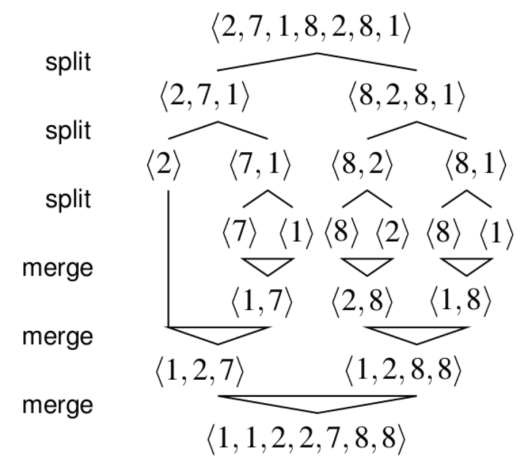
\includegraphics[height=6cm]{mergesort}
	\end{figure}
\end{frame}


\begin{frame}{Sortieren – Mergesort}
	\textbf{Laufzeit von Mergesort}
	\pause
	\begin{itemize}
		\item Es ist $T(n) = \begin{cases}
			1, & \text{falls } n \leq 1 \\
			2 \cdot T(\fract n/2 ) + c \cdot n, & \text{falls } n > 1
		\end{cases}$
		\pause
		\item \textbf{Master-Theorem}: \quad $T(n) \in \Theta(n \log n)$
		\pause
		\item Input ist ein \textbf{Array}? \impl  Schreibe Array in eine neue verkettete Liste, wende Mergesort an, kopiere Ergebnis zurück ins Array \\
		(\impl D.~h., Mergesort für Arrays ist \textbf{nicht in-place})
	\end{itemize}
\end{frame}

\begin{frame}{Aufgabe: Mergesort}
	\taskheading{Mergesort}
	Sortiert die Liste $\llist{65,12,42,87,5,42,33,29}$ mit Mergesort und zeichnet dazu den Rekursionsbaum.
\end{frame}

\begin{frame}{Aufgabe: Mergesort}
	\solutionheading
	\medskip
	\centering
	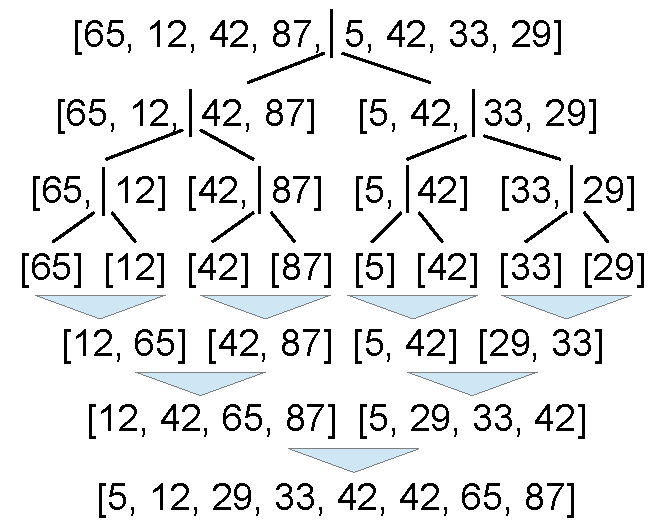
\includegraphics[height=.7\frameheight]{Mergesortaufgabe.pdf}
\end{frame}

\begin{frame}{Sortieren}
	\taskheading{Spaghettisort} 
	Unterm Schrank der Vorratskammer findet ihr noch einen guten Batzen (unzubereiteter, trockener) Spaghetti. Leider sind diese im Laufe der Jahre etwas brüchig geworden und liegen daher nun in sehr vielen verschiedenen Längen vor. Um einzuschätzen, ob ihr die Spaghetti noch essen wollt oder nicht, möchtet ihr das Durcheinander in eine übersichtlichere Anordnung überführen. \\
	\medskip
	Überlegt euch ein Verfahren, wie ihr die Nudeln in linearer Zeit (in Bezug auf die Anzahl der Spaghetti) der Länge nach sortieren könnt.
\end{frame}

\begin{frame}{Sortieren}
	\solutionheading 
	Die Spaghetti in der Hand auf dem Tisch aufrichten und „absacken“ lassen. Mit der anderen Hand von oben auf die Spaghetti herabfahren und so feststellen, welche Nudel zuerst piekst. Diese ist dann die Längste und wird links zu den bereits entfernten Spaghetti dazugelegt. Wiederholen, bis keine Spaghetti mehr unsortiert sind.
\end{frame}

\section{Untere Schranke $\Om{n \log n}$}

\begin{frame}[t]{Sortieren – untere Schranke}
	\textbf{Vorlesung}: \\
	\quad Vergleichsbasiertes Sortieren von $n$ Elementen dauert $\Omega(n \log n)$. \\
	\pause
	\bigskip
	\textbf{Zutaten:} 
	\begin{itemize}[<+->]
		\item \textbf{Binärbaum}: Ein Baum, bei dem jeder Knoten \textbf{maximal zwei} Kindknoten besitzt.
		\item \textbf{Höhe} $h$ eines Binärbaums: Die \textbf{Länge} des längsten (wiederholungsfreien) Pfades von der \textbf{Wurzel} zu einem \textbf{Blatt} \\ {\small ($=$ Anzahl Kanten, über die man läuft)}. 
		\item Ein Binärbaum der Höhe $h$ hat \textbf{maximal} $2^h$  Blätter.
	\end{itemize}	
\end{frame}

\begin{frame}{Sortieren – untere Schranke}
	\textbf{Der Sortierbaum -- Aufbau}
	\begin{figure}[htp]
		\centering
		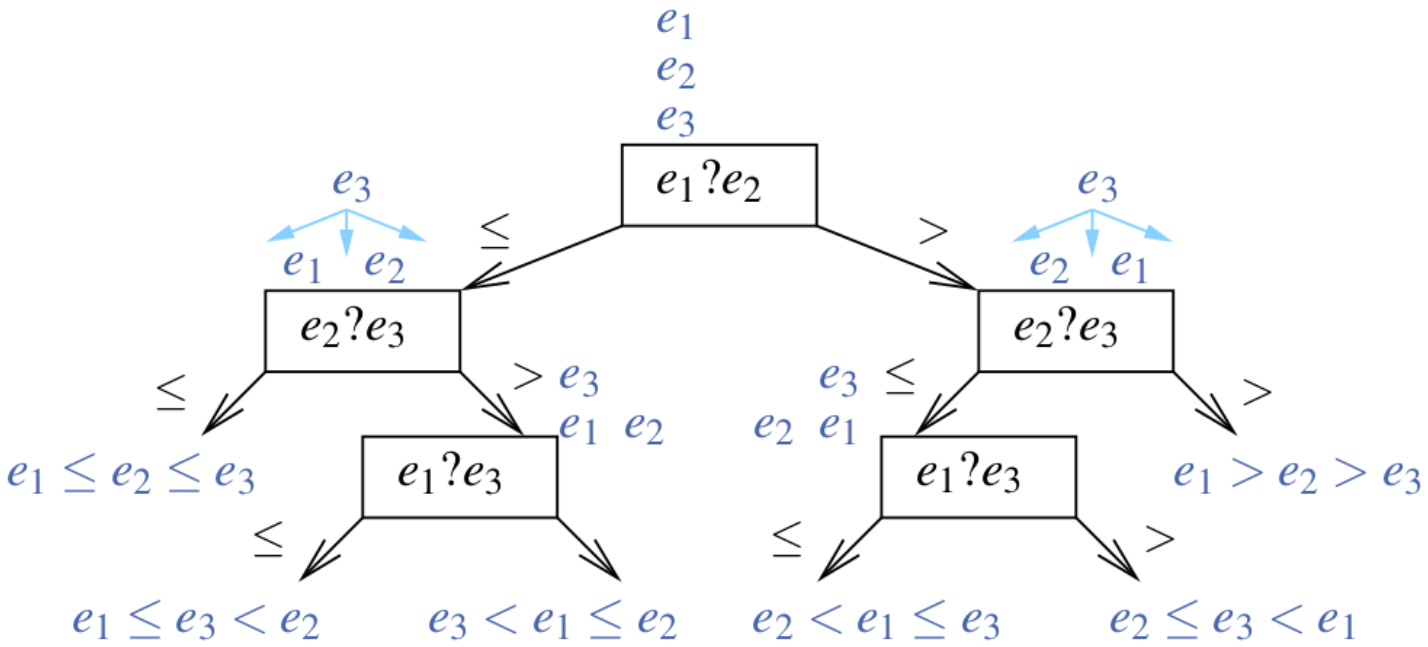
\includegraphics[width=11cm]{vergleichsbaum}
	\end{figure}
\end{frame}

\begin{frame}{Sortieren – untere Schranke}
	\textbf{Der Sortierbaum -- Funktionsweise}
	\begin{itemize}
	\item Für jede Folgenlänge $n$ gibt es einen \textbf{eigenen} Sortierbaum.
	\item Jeder \textbf{Knoten} im Baum repräsentiert den \textbf{Vergleich} zweier Elemente, dessen zwei mögliche Ergebnisse ($\leq$ oder $>$) zu versch. Kindern führen
	\implitem Ganz unten: \textbf{Blätter} repräsentieren \textbf{endgültige sortierte Reihenfolge} der Elemente (die durch die vorherigen Vergleiche bekannt ist)
	
	\pause
	\medskip
	\item Betrachte minimalen Sortierbaum $T$ für eine Folge der Länge $n$.
	\item Der Sortierbaum muss zu \textit{jeder möglichen Umsortierung} der Folge führen können \impl er \textbf{muss} $n!$ Blätter haben.
	\implitem Höhe $h_T \geq \log(n!)$
	\end{itemize}
\end{frame}



\begin{frame}[t]{Sortieren – untere Schranke}
	\textbf{Vorlesung}: \\
	\quad Vergleichsbasiertes Sortieren von $n$ Elementen dauert $\Omega(n \log n)$. \\
	\bigskip
	\textbf{Zutaten:} 
	\begin{itemize}
		\item \textbf{Binärbaum}: Ein Baum, bei dem jeder Knoten \textbf{maximal zwei} Kindknoten besitzt.
		\item \textbf{Höhe} $h$ eines Binärbaums: Die \textbf{Länge} des längsten (wiederholungsfreien) Pfades von der \textbf{Wurzel} zu einem \textbf{Blatt} \\ {\small ($=$ Anzahl Kanten, über die man läuft)}. 
		\item Ein Binärbaum der Höhe $h$ hat \textbf{maximal} $2^h$  Blätter.
		\item \alert{$\log(n!) \in \Theta(n\log n)$}
	\end{itemize}	
\end{frame}

\begin{frame}{Sortieren – untere Schranke}
	$\log(n!) \in O(n\log n)$, denn: 
	\pause
	\begin{align*}
		\log(n!) &= \log(1 \cdot 2 \cdot \cdots \cdot (n-1) \cdot n) \\
				 &\leq \log(n \cdot n \cdot \cdots \cdot \hphantom{(} n \hphantom{{\!}-1)} \cdot n) = \log(n^n) = n\log n.
	\end{align*}
	\pause
	
	$\log(n!) \in \Omega(n\log n)$, denn:
	\pause
	\begin{align*}
		\log(n!) 
		&= \log \Big( 
		\underbrace{1 \cdot 2 \cdots \cdot ( 
			\floor{\tfrac{n}{2}} - 1
			)}_{\visible<5->{\geq 1 \cdots 1}}     \cdot \floor{\tfrac{n}{2}} \cdot     \underbrace{( 
			\floor{\tfrac{n}{2}} + 1
			)  \cdots \cdot (n-1 ) \cdot n }_{\visible<5->{\geq \floor{\tfrac{n}{2}} \cdots \floor{\tfrac{n}{2}}}}
		\Big) \\
		\pause\pause
		&\geq \log \big( \overbrace{1 \cdot 1 \cdots\cdots\cdots\cdot 1 \cdot 1}      \cdot \floor{\tfrac{n}{2}} \cdot     \overbrace{\floor{\tfrac{n}{2}}  \cdots \cdots \cdots\cdots\cdots \floor{\tfrac{n}{2}} } \big) \\
		\pause
		& \geq \log\left(\floor{\frac{n}{2}}^{\floor{\frac{n}{2}}}\right) = \floor{\frac{n}{2}} \cdot \log\left(\floor{\frac{n}{2}}\right) \\ 
		\pause
		& \in \Th{\frac{1}{2} \cdot n \cdot (\log n - \log 2 )} = \Theta(n \log n)
	\end{align*}
\end{frame}

\begin{frame}{Sortieren – untere Schranke}
\textbf{Der Sortierbaum -- Analyse}
\begin{itemize}
	\item Höhe $h_T \geq \log(n!) \in \Theta(n \log n)$ 
	\item Höhe $h_T \entspr$ Anzahl nötiger \textbf{Vergleiche} \entspr (Worst-Case-)\textbf{Laufzeit}
	\Implitem Vergleichsbasierte Sortieralgorithmen können keinen besseren Worst-Case als $\Theta(n\log n)$ haben.
	\implitem \textbf{untere asymptotische Schranke} für vergleichsbasiertes Sortieren, „schneller geht's nicht“. \quad\qedsymbol
\end{itemize}
\end{frame}

%\begin{frame}{Sortieren – untere Schranke}
%	\textbf{Vorbereitende Definitionen}
%	\pause
%	\begin{itemize}
%		
%		\pause
%		\item \textbf{Wurzel}: Knoten eines Baumes, der keine Eltern hat.
%		\item \textbf{Blatt}: Knoten eines Baumes, der keine Kinder hat.
%		\pause
%		
%	\end{itemize}
%\end{frame}

%\begin{frame}{Sortieren – untere Schranke}
%	\textbf{Behauptung}: Ein Binärbaum der Höhe $h$ hat \textbf{maximal} $2^h$  Blätter. \\
%	\pause
%	\textbf{Beweis} durch vollständige Induktion über $h$: \\
%	\pause
%	\hanging {\textbf{IA}. ($h = 0$):  \quad $T$ mit $h = 0$ hat nur einen Knoten: Wurzel $=$ Blatt. \newline $2^0 = 1$ \ \checkmark } \\
%	\pause
%	\hanging {\textbf{IV}.: Für ein festes $h \in \N_0$ gelte die Behauptung für alle Binärbäume der Höhe $h' \leq h$.} \\
%	\pause
%	\hanging {\textbf{IS}. ($h \rightsquigarrow h+1$): \quad Sei $T$ Binärbaum mit Höhe $h+1$ und Wurzel $w$. $w$ hat maximal 2 Kinder. Beide sind Wurzeln kleinerer Sub-Bäume $S_1, S_2$. Die $S_k$ haben max. Höhe $h$ $\stackrel{\text{IV}}{\impl}$ haben max. $2^h$ Blätter. \newline
%		\Impl $T$ hat insges. max. $2 \cdot 2^h = 2^{h+1}$ Blätter. \qed } \\
%	%Betrachte den Wurzelknoten des Binärbaumes der Höhe $h+1$. Dieser hat maximal zwei Kindknoten. Jeder dieser Kindknoten ist Wurzelknoten eines (Sub-)Baumes der maximalen Höhe $h$ und führt (nach IV.) somit jeweils maximal zu $2^h$ Blattknoten. \\
%	%Der gesamte Binärbaum hat also insgesamt maximal $2 \cdot 2^h = 2^{h+1}$ Blattknoten. 
%	\pause
%	\impl \textbf{Folgerung}: Ein Binärbaum mit $n$ Blättern muss \textit{mindestens} die Höhe $\log n$ haben.
%\end{frame}

\begin{frame}{The Sound of Sorting}
	\url{http://panthema.net/2013/sound-of-sorting/}
\end{frame}


\begin{frame}{Sortieren}
	\taskheading{Doktor Meta is back!} 
	{	\small
		Der ebenso geniale wie hochmoderne Superbösewicht Doktor Meta ist in Aufbruchstimmung! Erst neulich hat er eine klaffende Marktlücke erkannt, mit der er seinen Reichtum mehren und schließlich die Weltherrschaft an sich reißen wird: Den Verleih von \textbf{Turingmaschinen}!
		
		Zur Zeit besitzt Doktor Meta $k \in \N$ unterschiedliche Typen von TMen. Von jedem Typ $t \in \{1 ... k\}$ sind $c_t$ Stück vorhanden, die alle verliehen werden können. Seine Buchungsanfragen-TM ist jedoch von seinem größten Widersacher Turing-Man (halb Mensch, halb Turingmaschine) entwendet worden, um den Superbösewicht zu stoppen. 
		
		Somit liegen also $n$ Buchungen vor (bestehend aus \emph{Abholzeitpunkt}, \textit{Rückgabezeitpunkt} und \emph{Typ} der TM) und es muss möglichst schnell (und natürlich algorithmisch) entschieden werden, ob die vorliegenden Buchungen alle erfüllt werden können.	
			
		%Stets hat man ihn als realitätsfern belächelt, doch jetzt sieht Mister X seinen Triumph gekommen: Als Spezialist der Theoretischen Informatik hat er den Ruf der Zukunft vernommen und beschlossen, die nächste Stufe der Modernisierung einzuleiten. Schließlich hat er in seiner nicht endenden Genialität eine klaffende Marktlücke erkannt und direkt ein Monopol mit dem Verleih von Turingmaschinen (TM) aufgebaut. Gerade eröffnet er zwar erst seine erste Filiale, doch schon bald wird er expandieren, ein Imperium errichten und die Weltherrschaft erlangen!! Oder zumindest plant er das. \\
		%Zur Zeit besitzt er $k \in \N$ unterschiedliche Arten von TMen. Von jedem Typ $t \in \{1 ... k\}$ sind $c_t$ TMen vorhanden, die alle verliehen werden können. Leider konnte die TM, die Mister X zur automatisierten Anfragebeantwortung einsetzt, ihr Entscheidungsproblem nicht lösen und hat daher sämtliche Anfragen mit „ja“ beantwortet. Nun liegen also $n$ Buchungen (bestehend aus Abholzeitpunkt, Rückgabezeitpunkt und Art der TM) vor und es muss möglichst schnell (und natürlich algorithmisch) entschieden werden, ob die vorliegenden Buchungen alle erfüllt werden können. \\
		Entwerft einen Algorithmus, der dieses Problem in höchstens $O(n \log n + k)$  löst.
		(Geht davon aus, dass eine TM sofort wieder verliehen werden kann, sobald sie zurückgegeben wurde.)
	}
\end{frame}

\begin{frame}{Sortieren}
	\solutionheading
	\vspace{-.4\baselineskip} \textbf{Konvertiere} Buchungsliste $\rightsquigarrow$ Liste von \textbf{Ereignissen}: $\left(\stackedtight{\text{Zeitpunkt } \\ \text{Typ }t \\ dx}\right)$, \\ 
	\vspace{-.8\baselineskip} wobei $dx = \tight{\caseslr{-1 & \text{für Ausleihe} \\ 1 & \text{für Rückgabe}}}$. \\
	\impl Für jede Buchung werden \textbf{zwei} Ereignisse angelegt. \\
	\textbf{Sortiere} Ereignisliste aufsteigend nach Zeitpunkt (falls gleiche Zeit \impl Rückgabe \textbf{vor} Ausleihe!) \\
	\textbf{Initialisiere} $A: \KwArray A[1...k] \KwOf \Z$ \quad mit \quad  $A[t] := c_t \quad \forall t=1..k$. \\
	\For{$e \KwIn \text{Ereignisse}$}{
		$A[e.t] \pluseq e.dx$ \\
		\If{$A[e.t] < 0$}{
			\Return{\KwFalse} \RComment{unerfüllbar} \;
		}
	}
	\Return{\KwTrue} \RComment{erfüllbar} \\
	\textbf{Laufzeit}: Sortieren von $2n$ Ereignissen: $O(n \log n)$ (mit Mergesort), Initialisieren von $A$ in $O(k)$. Rest: $O(n)$ \Impl \textbf{insgesamt} $O(n \log n + k)$.
	
	
	%Zunächst wird aus der Liste der Buchungen eine Liste von Ereignissen erzeugt. Ein Ereignis besteht aus einem Zeitpunkt, dem Typ $t$ der TM und einer Zahl $dx$, die bei Ausleihe $-1$ und bei Rückgabe $1$ ist, d.h. für jede Buchung werden genau zwei Ereignisse angelegt. Die Liste der Ereignisse wird dann aufsteigend nach Zeitpunkt sortiert, wobei bei Ereignissen mit gleichen Zeitpunkten Rückgaben vor Ausleihen sortiert werden müssen. \\
	%Lege dann ein $\KwArray A[1...k] \KwOf \Z$ an, wobei $A[t] := c_t$ initialisiert wird. Iteriere danach über $e \in$ Ereignisliste und addiere $e.dx$ auf $A[e.t]$. Wird ein $A[t]$ zu einem beliebigen Zeitpunkt kleiner $0$, sind die Buchungen unerfüllbar, ansonsten schon. \\
	%Das Sortieren von $2n$ Ereignissen liegt in $O(n\log n)$ (z.B. mit Mergesort), das Anlegen von $A$ in $O(k)$. Der Rest liegt in $O(n)$, also insgesamt $O(n\log n + k)$ Laufzeit.
\end{frame}

\xkcdframe{1185}{Danke für eure Aufmerksamkeit! \smiley}{0}

\only<beamer:0>{\slideThanks}

\end{document}